\documentclass[runningheads]{llncs}
\usepackage{graphicx}
\usepackage{amsmath,amssymb} % define this before the line numbering.
\usepackage{color}
\usepackage{censor}
% See
% https://stackoverflow.com/questions/1061112/eliminate-space-before-beginitemize
% Lots of authors seem to hate the spacing before lists in LaTeX. nolistsep
% takes it out.
\usepackage{enumitem}
%\setlist{nolistsep}

%===========================================================
% Custom commands
\newcommand{\mat}{\mathbf}
\DeclareMathOperator{\pa}{pa}
\DeclareMathOperator{\argmin}{arg min}

% For final copy (from WACV style)
\newif\ifaccvfinal{}
\accvfinalfalse{}
\def\accvfinalcopy{\global\accvfinaltrue}
% Here's how you enable final copy styles (be careful of the acknowledgements!)
% \accvfinalcopy{}

\ifaccvfinal\else
\usepackage{ruler}
\fi

%===========================================================
\begin{document}
\pagestyle{headings}
\mainmatter{}

\ifaccvfinal\else
\def\ACCV16SubNumber{***}  % Insert your submission number here
\fi

%===========================================================
\title{Exploiting Temporal Relationships for Human Pose Estimation using Biposelets}
\ifaccvfinal{}
    \author{Sam Toyer\\\texttt{u5568237@anu.edu.au}}
    \institute{Australian National University}
\else
    \titlerunning{ACCV-16 submission ID \ACCV16SubNumber}
    \authorrunning{ACCV-16 submission ID \ACCV16SubNumber}

    \author{Anonymous ACCV 2016 submission}
    \institute{Paper ID \ACCV16SubNumber}
\fi

\maketitle

%%%%%%%%%%%%%%%%%%%%%%%%%%%%%%%%%%%%%%%%%%%%%%%%%%%%%%%%%%%%%%%%%%%%%%%%%%%%%%%
% Misc formatting notes:
%
% - Use "This is not a pipe~\cite{sourceYY}." to cite papers (not fancy natbib
%   stuff)
% - They want punctuated equations and a ~ space between the end of the equation
%   and the punctuation (either comma or full stop).
% - Don't feel obligated to go to 14 pages. A quick skim of accepted papers from
%   ACCV 2014 shows that going above 10 pages is the norm (shortest I saw was 12
%   pages), but that fewer than 14 pages of actual content is totally
%   acceptable.
% - Structure is flexible. For instance:
%   - There's no need for a separate discussion section (apart from discussion
%     in experiments section)
%   - Some authors don't include a separate section for related work, some do.
%   - Long sections are acceptable (but poor practice, IMO)

%%%%%%%%%%%%%%%%%%%%%%%%%%%%%%%%%%%%%%%%%%%%%%%%%%%%%%%%%%%%%%%%%%%%%%%%%%%%%%%
% Tentative list of figures to produce:
%
% - One flow chart for the entire pose estimation process (re-use images from
%   PowerPoint, but in Inkscape or something that plays nicely with LaTeX)
% - Big panel of biposelets
% - Illustration of stitching model for single frames (much like the one in my
%   PowerPoint)
% - Possibly a small summary figure at the beginning showing some representative
%   detections to lend flavour to the rest of the paper.
% - Possibly a CNN architecture diagram showing how flow is merged with RGB
%   images---would prefer not to do that, since it's not a well-explored aspect
%   of my approach. If I do choose to do that, I can probably stick to boxes to
%   represent the CNN layers, with some images of RGB input and flow on one side
%   and biposelets on the other
% - Panels of good at bad predictions for MPII Cooking Activities, Poses in the
%   Wild and H3.6M
% - Plots of PCK and strict PCP:
%   - Raw PCK for Poses in the Wild
%   - PCP-strict at various thresholds for PIW (include table for PCP@0.5)
%   - PCP-strict at various thresholds for MPII Cooking Activities (also needs
%     table for PCP@0.5)
%   - PCKh for H3.6M in same format as recurrent convnet paper

%%%%%%%%%%%%%%%%%%%%%%%%%%%%%%%%%%%%%%%%%%%%%%%%%%%%%%%%%%%%%%%%%%%%%%%%%%%%%%%
% Page budgeting (14 page content limit with unlimited references):
%
% - 1 page for introduction, abstract and title
% - 1-2 pages for related work
% - 4-5 pages for method (frame pair model + stitching + learning)
% - 5-6 pages for experiments and discussion (depending on space available)
% - 0.5 pages for conclusion and acknowledgement

\begin{abstract}
The problem of human pose estimation in still images has been well-studied in
recent years, but making effective use of the temporal information inherent in
videos is still an open problem. We propose a new model which attempts to learn
temporal relationships by using a CNN to predict poses for several frames at a
time; our model caters to the detection capabilities of CNNs by casting pose
estimation as a problem of predicting the \textit{biposelets} which poses in
adjacent frames are composed of. Predicting poses in two frames at a time
reduces pose estimation over an entire video sequence to the problem of choosing
a pose for each frame from a set of high-scoring poses, which can be achieved by
minimising a trivial pairwise cost with dynamic programming. Experiments show
that our approach performs competitively with existing approaches on established
pose estimation benchmarks.
\end{abstract}

\section{Introduction}

% TODO: Why pose estimation in general is interesting:
%  - Challenging task in general
%  - Use it for 3D pose estimation
%  - Use it for action recognition (P-CNN paper is relevant example)
%  - Use it for just about everything else
Human pose estimation aims to recover the locations of a person's joints from
images of the person. %TODO
2D pose estimation is also useful as a preprocessing step for higher-level
vision tasks, including 3D pose
estimation~\cite{andriluka2010monocular,zhou2016spatio} and action
recognition~\cite{cheron2015p,yao2011does}.

% TODO: Why video pose estimation in particular is interesting:
%  - Few results so far (--> is this true? There seem to be lots of results, but
%    they're just dwarfed by the number of static pose estimation papers!)
%  - Intuitively seems like temporal information should lead to big improvement
%  - Hard to actually get solid improvement in practice
Intuitively, pose estimation in videos ought to be more effective than pose
estimation in static images. Even if a pose is blurred or occluded in one frame
of a video, it is often possible for humans to approximate it well by making use
of the context provided by surrounding frames.

% TODO: How we approach the problem; briefly summarise the biposelet detection
% and sequence stitching stages here.

\section{Related work}

Pose estimation methods for static images typically build on an appearance model
which can be applied in a sliding window fashion to locate joints. Linear
classifiers applied to histogram-of-gradients features are commonly used for
this purpose~\cite{yang2011articulated,cherian2014mixing}, but have been
eclipsed by increasingly sophisticated convolutional network
architectures~\cite{jain2014modeep,tompson2014joint,chen2014articulated,pfister2015flowing,wei2016convolutional},
and our appearance model reflects this trend.

Appearance models can be complemented by global constraints on the relative
positions of joints. For instance, Yang and Ramanan~\cite{yang2011articulated}
define a graphical model which encourages joint locations to fall in regions of
the image with high appearance scores while penalising atypical limb lengths and
orientations. Several approaches also use the appearance of body parts to infer
``types'' which characterise those parts' positions relative to their
neighbours~\cite{yang2011articulated,chen2014articulated}. Our approach is
similar, although we break with past work by attempting to simultaneously
localise entire subsets of a person's joints instead of a single joint at a
time.

In videos, pose estimation is frequently accomplished using a
tracking-by-detection approach in which a set of poses is estimated
independently for each frame of the video and then combined into a single
temporally coherent
sequence~\cite{andriluka2010monocular,ferrari2008progressive,cherian2014mixing,ramanan2005strike}.
Our work follows a similar pattern, except we perform pose estimation at the
level of frame pairs instead of individual frames. Predicting pairs of poses
makes it simple to combine our set of detections for each frame pair into a
sequence of poses for each frame, as described in Section~\ref{sec:stitching}.
In contrast, past work using the frame-at-a-time method has had to resort to
more complex flow- and appearance-based heuristics to ensure temporal
consistency between predicted poses~\cite{cherian2014mixing}.

There have been several attempts to exploit motion information at the network
level: MoDeep~\cite{jain2014modeep} simply augmented a heatmap regressor for
joint positions with ``motion features'' derived from the frame for which a pose
was being predicted and the one prior to it. For localisation of fast-moving
joints, the authors reported a boost in performance over an equivalent model
without motion features, but little boost in performance for slower-moving
joints like the elbows. This suggests that an understanding of the temporal
relationships between joint positions is either unhelpful to pose estimation or
was not being learnt effectively.

% TODO: Do I actually show that the recurrent approach is inferior? I should be
% able to, but if I can't then I need to change this.
Other approaches to learning temporal relationships at the network level include
the ``flowing convnets''~\cite{pfister2015flowing} and the recurrent networks of
Fragkiadaki et al.~\cite{fragkiadaki2015recurrent}. The former approach achieved
state-of-the-art accuracy by using optical flow to backwarp joint position
heatmaps to adjacent frames, then pooling the heatmaps to produce a final pose
estimate; nevertheless, its ``learning'' of temporal relationships was limited
to choosing a set of pooling weights for combining backwarped heatmaps. The
latter approach attempted to make use of information from adjacent frames using
a recurrent architecture which included LSTM nodes, but failed to achieve
state-of-the-art performance, as our experiments in
Section~\ref{sec:experiments} show.

\section{Detecting pose pairs}

% What I want to say:
% - (✓) Objective of this stage of pipeline is to find a pose in each frame of each
%   neighbouring frame pair.
% - (✓) Decompose pose into several subposes.
% - (✓) Intuitively: want to predict a configuration (poselet) for each subpose.
%   Choose configurations by applying K-means to all relative positions. This is
%   tied to the CNN training step, so I will have to explain it there.
% - (✓) In our method: each configuration gives a location for each joint within
%   both frames. This allows configurations to capture both location and motion.
%   Call these configurations biposelets.
% - (✓) NOW talk about cost function.
% - (✓) Talk about pairwise costs and how the means are found for the pairwise
%   costs.
% - Need to mention optical flow implementation in use.
% - (✓) Talk about maximising cost function.
%   - Just message passing with distance transforms.
%   - Need complexity mentioned in there somewhere.
% - How unaries are produced and learnt by CNN (one follows from the other):
%   - CNN architecture
%   - CNN input (two frames + flow between them)
%   - CNN output
%   - CNN objective.
%   - Fully convolutional inference
%   - Learning (just SGD) --> maybe put the training details in the experiments
%     section.
% - How SSVM is learnt. Talk about learning target, how positives/negatives are
%   used, where supervision comes in (if anywhere), how things are optimised
%   (just cite ramanan2013dual). <-- Maybe put in learning section
% - (✓) How poses are recovered from a set of subpose locations and types for
%   each subpose.

\subsection{Subposes and biposelets}\label{sec:decomp}

In the first stage of our pipeline, we consider each neighbouring pair of frames
in a sequence and simultaneously infer the poses present in each. For the
purposes of this stage, we decompose a pair of poses in neighbouring frames into
a fixed set of subposes, each of which correspond to a subset of joints in the
original pose. Subposes are chosen so that each subpose shares exactly a joint
with at least one neighbouring subpose, and each joint in the original pose is
present in at least one subpose. For instance, a pose containing shoulder, elbow
and wrist joints could be decomposed into one subpose containing wrist and elbow
joints on the left side of the body, one subpose containing elbow and shoulder
joints on the left hand side, one subpose containing both the left and right
shoulders, etc.

Rather than representing the locations of each joint in each subpose directly,
we discretise the space of configurations for joints within each subpose into
$K$ \textit{biposelets}. Biposelets are so named in analogy to the
\textit{poselets} of Bourdev and Malik~\cite{bourdev2009poselets}. Unlike their
namesake, however, biposelets give a position for each joint in a subpose across
two video frames instead of a single one. This allows biposelets to represent
both the relative positions of joints and their movement over time. A
representative set of biposelets learnt for the MPII Cooking Activities pose
estimation dataset~\cite{rohrbach2012database} is shown in
Figure~\ref{fig:biposelets}.

\begin{figure*}[t]
\begin{center}
\begin{tabular}{@{}c@{}c@{}c@{}c@{}c@{}c@{}c@{}c@{}}
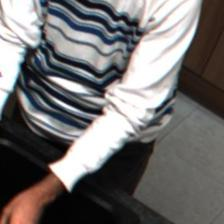
\includegraphics[height=0.1375\linewidth]{figures/biposelets/poselet-230/sample-1-f0.jpg}\,&
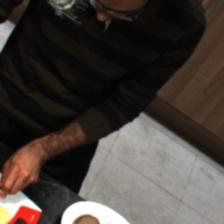
\includegraphics[height=0.1375\linewidth]{figures/biposelets/poselet-230/sample-2-f0.jpg}\,&
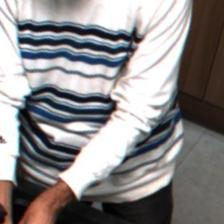
\includegraphics[height=0.1375\linewidth]{figures/biposelets/poselet-230/sample-3-f0.jpg}\,&
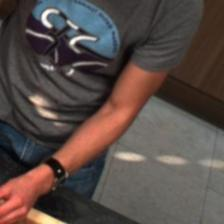
\includegraphics[height=0.1375\linewidth]{figures/biposelets/poselet-230/sample-4-f0.jpg}\,&
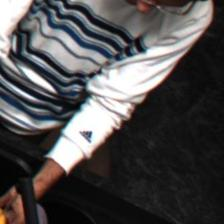
\includegraphics[height=0.1375\linewidth]{figures/biposelets/poselet-230/sample-5-f0.jpg}\,&
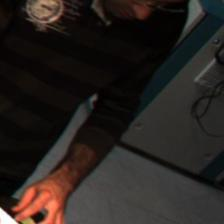
\includegraphics[height=0.1375\linewidth]{figures/biposelets/poselet-230/sample-6-f0.jpg}\,&
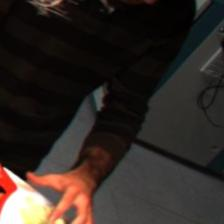
\includegraphics[height=0.1375\linewidth]{figures/biposelets/poselet-230/sample-7-f0.jpg}\\
%
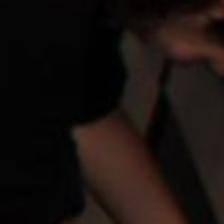
\includegraphics[height=0.1375\linewidth]{figures/biposelets/poselet-289/sample-1-f0.jpg}\,&
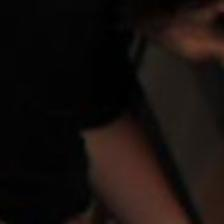
\includegraphics[height=0.1375\linewidth]{figures/biposelets/poselet-289/sample-2-f0.jpg}\,&
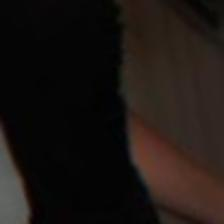
\includegraphics[height=0.1375\linewidth]{figures/biposelets/poselet-289/sample-3-f0.jpg}\,&
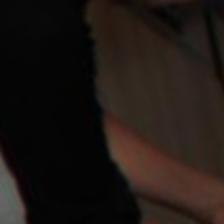
\includegraphics[height=0.1375\linewidth]{figures/biposelets/poselet-289/sample-4-f0.jpg}\,&
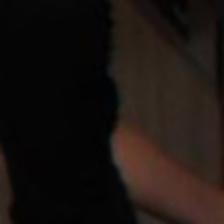
\includegraphics[height=0.1375\linewidth]{figures/biposelets/poselet-289/sample-5-f0.jpg}\,&
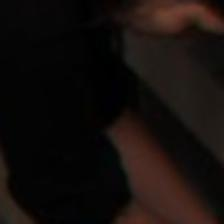
\includegraphics[height=0.1375\linewidth]{figures/biposelets/poselet-289/sample-6-f0.jpg}\,&
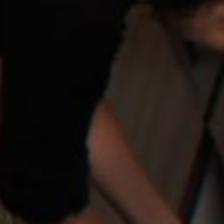
\includegraphics[height=0.1375\linewidth]{figures/biposelets/poselet-289/sample-7-f0.jpg}\\
%
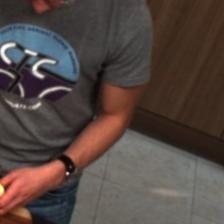
\includegraphics[height=0.1375\linewidth]{figures/biposelets/poselet-297/sample-1-f0.jpg}\,&
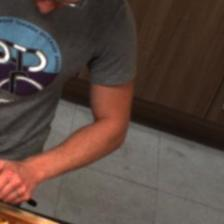
\includegraphics[height=0.1375\linewidth]{figures/biposelets/poselet-297/sample-2-f0.jpg}\,&
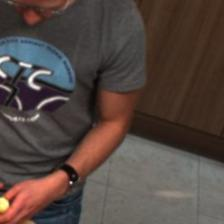
\includegraphics[height=0.1375\linewidth]{figures/biposelets/poselet-297/sample-3-f0.jpg}\,&

\includegraphics[height=0.1375\linewidth]{figures/biposelets/poselet-297/sample-4-f0.jpg}\,&
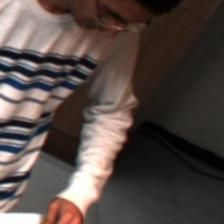
\includegraphics[height=0.1375\linewidth]{figures/biposelets/poselet-297/sample-5-f0.jpg}\,&
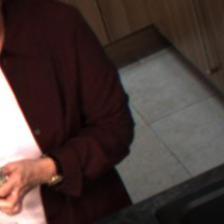
\includegraphics[height=0.1375\linewidth]{figures/biposelets/poselet-297/sample-6-f0.jpg}\,&
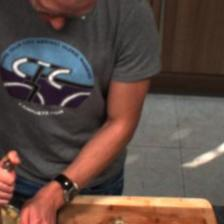
\includegraphics[height=0.1375\linewidth]{figures/biposelets/poselet-297/sample-7-f0.jpg}\\
\end{tabular}
\end{center}
\caption{Biposelets learnt for left elbows in the MPII Cooking Activities
dataset. Different rows show different biposelets. For brevity,
only the first frame associated with each biposelet is shown.}
\label{fig:biposelets}
\end{figure*}

% TODO: Give motivation for decomposing into subposes and biposelets instead of:
% 1) Considering a single joint at a time
% 2) Considering the entire pose

\subsection{Frame pair model}

Formally, our frame pair model conceptualises a pose as a tree-structured graph
$\mathcal G = (\mathcal S, \mathcal E)$ consisting of a set of subposes
$\mathcal S$ and a set of edges $\mathcal E \subset \mathcal S \times \mathcal
S$. Subposes are chosen according to the constraints listed in
Section~\ref{sec:decomp}, and a pair of subposes $(s_1, s_2)$ will have an edge
between them iff they have a joint in common. The objective of the first stage
of our pipeline is to take a pair of frames $(\mat I_1, \mat I_2)$ and output,
for each subpose $s$, a subpose location $\vec l_s \in \mathbb R^2$ within the
frame pair and a biposelet type $t_s \in \{1, \ldots, K\}$. Specifically, the
first stage must find some $\mat L = \begin{bmatrix}\vec l_1 & \vec l_2 & \cdots
& \vec l_{|\mathcal S|}\end{bmatrix}^T$ and $\vec t = \begin{bmatrix}t_1 & t_2 &
\cdots & t_{|\mathcal S|}\end{bmatrix}$ which minimises the cost
%
\begin{equation}\label{eqn:full-cost}
C(\mat L, \vec t \mid \mat D_{12})
= w_0 + \sum_{s \in \mathcal V} \phi_s(\vec l_s, t_s; \mat D_{12})
+ \sum_{(s_1, s_2) \in \mathcal E}
    \psi_{s_1 s_2}(\vec l_{s_1}, \vec l_{s_2}, t_1, t_2)~,
\end{equation}
%
where $w_0$ is a bias, each $\phi_s(\cdot)$ is an appearance term, each
$\psi_{s_1,s_2}$ is a pairwise cost, and $\mat D_{12}$ is the concatenation
of $\mat I_1$ and $\mat I_2$.

Recall that each pair of neighbouring subposes have a single joint in common;
the aim of the pairwise terms is to ensure that locations of neighbouring
subposes are chosen so that predicted locations for their shared joints are
consistent. Concretely, each pairwise cost can be written out in full as
%
\begin{equation}\label{eqn:pair-cost}
\psi_{s_1 s_2}(\vec l_{s_1}, \vec l_{s_2}, t_1, t_2)
= \langle
    \vec w_{s_1 s_2},
    \vec \Delta(\vec l_{s_1} - \vec l_{s_2}  - \vec m_{t_1 t_2})
\rangle~,
\end{equation}
%
where $\vec \Delta(\begin{bmatrix}\delta_x & \delta_y\end{bmatrix}) =
\begin{bmatrix}\delta_x^2 & \delta_x & \delta_y^2 & \delta_y\end{bmatrix}$ is a
deformation feature, $\vec w_{s_1 s_2}$ is a learnt weight vector, and
$\vec m_{t_1 t_2}$ is an ``ideal'' displacement between $s_1$ and $s_2$. If the
joint shared between $s_1$ and $s_2$ is at location $\vec r_{t,f}$ in frame $f$
and biposelet $t$ (relative to the centre of the biposelet), then $\vec m_{t_1
t_2}$ is simply
\begin{equation}
\frac{%
    \left(\vec r_{t_2,1} - \vec r_{t_1,1}\right)
    + \left(\vec r_{t_2,2} - \vec r_{t_1,2}\right)
}{2}~.
\end{equation}

Each appearance term $\phi_s(\vec l_s, t_s; \mat D_{12})$ reflects the degree to
which a small region around the location $\vec l_s$ looks like the subpose $s$
of type $t$. Concretely,
\begin{equation}\label{eqn:unary-cost}
\phi_s(\vec l_s, t_s; \mat D_{12}) = -w_s \log p(s, t_s \mid \mat D_{12}(
\vec l_s))~,
\end{equation}
%
where $w_s$ is a learnt weight and $\mat D_{12}(\vec l_s)$ denotes a crop of the
frame pair $(\mat I_1, I_2)$ and the optical flow between them at location
$\vec l_s$. $p(s, t \mid \mat D(\vec l))$ is the probability that the patch
$\mat D(\vec l)$ contains a subpose $s$ with biposelet $t$, with the special
values $(s, t) = (0, 0)$ denoting a background patch with no subpose.

% TODO: Should consider motivating design decision instead of just documenting
% it
$p(s, t \mid \mat D(\vec l))$ is produced by a two-stream convolutional neural
network with an architecture loosely following the 16 layer architecture of
Simonyan et al.~\cite{simonyan2014very}. Specifically, we use a two-stream
architecture in which one stream processes a stacked pair of RGB video frames
and another stream processes the flow; the two streams are merged by
concatenating them after the third pooling layer. The output is a probability
distribution over all subposes $s$ and biposelets $t$ for each subpose, with the
aforementioned special values of $(s, t) = (0, 0)$ denoting the background
class.

At test time, we efficiently apply the network as a sliding window detector by
converting the final dense layers to produce a fully convolutional
network~\cite{sermanet2013overfeat}. Section~\ref{sec:learning} discusses
training-time considerations.

% Reference for flow: Brox et al.~\cite{brox2004high}

\subsection{Inference on frame pair model}

The full cost (\ref{eqn:full-cost}) can be minimised efficiently by exploiting
the subpose graph's tree structure. For each subpose $s$, define the minimal
cost of the subtree rooted at $s$ as
%
\begin{equation}\label{eqn:reccost}
\begin{split}
M(\vec l_s, t_s; \mat D_{12}) =
&\sum_{s' : \pa(s') = s} \min_{\vec l_{s'}, t_{s'}} \left(\psi_{s s'}(\vec l_s,
\vec l_{s'}, t_s, t_{s'}) + M(\vec l_{s'}, t_{s'}; \mat D_{12})\right)
\\&\quad+ \phi_s(\vec l_s, t_s; \mat D_{12})~,
\end{split}
\end{equation}
%
where $\vec l_s$ and $t_s$ are the location and biposelet type, respectively, of
$s$, and $\pa(s') = s$ iff subpose $s$ is the parent of subpose $s'$ in
$\mathcal G$.

$M$ can be calculated for each location and type of the root subpose by
proceeding from the leaves of $\mathcal G$ upwards: for each leaf subpose $s_l$,
$M(\vec l_{s_l}, t_{s_l}; \mat D_{12})$ is simply $\phi_{s_l}(\vec l_{s_l},
t_{s_l}; \mat D_{12})$. For a non-leaf subpose $s$, $M(\vec l_s, \vec t_s; \mat
D_{12})$ can be computed by first evaluating $M(\vec l_{s_c}, t_{s_c}; \mat
D_{12})$ for each child $s_c$ of $s$, then applying Felzenszwalb and
Huttenlocher's distance transform technique~\cite{felzenszwalb2012distance} to
find the $\vec l_{s_c}$ which minimises $\psi_{s s_c}(\vec l_s, \vec l_{s_c},
t_s, t_{s_c})$ for each $t_{s_c}$. If there are $N$ locations in the image and
$K$ possible values for $t_{s_c}$ and $t_s$, then this will take $\mathcal O(N
K^2)$ time for each child and each $\vec l_s$; repeating the procedure for all
subposes in $\mathcal G$ thus takes $\mathcal O(|\mathcal S| N K^2)$ time.

Having evaluated (\ref{eqn:reccost}) for each possible $\vec l_{s_R}$ and
$t_{s_R}$, finding the pose configuration which minimises (\ref{eqn:full-cost})
is a simple matter of looking up
%
\begin{equation}
\argmin_{\vec l_{s_R}, t_{s_R}} M(\vec l_{s_R}, \vec t_{s_R}; \mat D_{12})
\end{equation}
%
and then backtracking to recover the locations and types of all other subposes.
This backtracking process can be repeated for several root locations and types
to produce a set of low-cost pose configurations for each frame pair; having
several such configurations is important during the sequence stitching stage of
the pipeline, as explained in Section~\ref{sec:stitching}.

After determining a location and biposelet type for each subpose, we can recover
a location for each joint in the original pose model using the stored joint
offsets associated with each assigned biposelet. In cases where two subposes
share a joint, the final joint location is the average of the joint locations
predicted by the biposelets associated with the two subposes.

\section{Sequence stitching}\label{sec:stitching}

% TODO: Might need some more motivation here. There's an interesting comparison
% with Anoop's past work to be made, but I haven't written it yet :P

After evaluating the first stage of our pipeline on every frame pair in a video
sequence, we obtain a small candidate set of pose pairs for each frame pair. The
second stage of the pipeline attempts to pick a single pose pair from each
candidate set of pose pairs, then combines poses from overlapping pairs to obtain
a single pose for each frame. Chosen pose pairs should meet two criteria:
%
\begin{description}
\item[Individual plausibility] Low cost poses, in the sense of the cost
function (\ref{eqn:full-cost}) for the frame-pair model, should be preferred over
high cost ones.
\item[Temporal consistency] Where two selected pose pairs overlap on a frame,
the selected poses for that frame should be similar.
\end{description}

The pair selection criteria are easy to express mathematically. For a sequence
of $F$ frames, let $\mathcal P_f$ denote the set of pose pairs detected between
frame $f$ and $f + 1$, where $f \in \{1, \ldots, F - 1\}$. Further, let $(\mat
p_{f,1}, \mat p_{f_2})$ denote the specific pose pair which the sequence
stitcher chooses from set $\mathcal P_f$, and $c_f$ be cost
(\ref{eqn:full-cost}) associated with the subpose locations and types defining
that pose pair. The objective of the stitcher is to find a sequence of pose
pairs $(\mat p_{1,1}, \mat p_{1,2}), (\mat p_{2,1}, \mat p_{2,2}), \ldots, (\mat
p_{f-1,1}, \mat p_{f-1,2})$ from the sets $\mathcal P_1, \mathcal P_2, \ldots,
\mathcal P_{F-1}$ which minimises
%
\begin{equation}\label{eqn:stitch-cost}
\sum_{f=1}^{F-1} \|\mat p_{f,2} - \mat p_{f+1,1}\|_2^2
+ \lambda \sum_{f=1}^{F-1} c_f~.
\end{equation}
%
The first term encourages temporal consistency, whilst the second favours
low-cost pose pairs over high-cost ones. $\lambda$ is a constant which balances
the two considerations.

Once an appropriate sequence of pose pairs has been chosen, a final pose may be
produced for each frame frame $1 < f < F$ by averaging $\mat p_{f-1,2}$ and
$\mat p_{f,1}$. In the first and last frames, there will only be one selected
pose to begin with, as there is only one pose pair associated with each of those
frames.

The stitching cost (\ref{eqn:stitch-cost}) can be efficiently minimised using a
dynamic programming approach analogous to the Viterbi algorithm. If there are
$|\mathcal P|$ pose pairs in each candidate set, then this maximisation will
take $\mathcal O(|\mathcal P|^2)$ time. Thus, it is important to produce only a
small selection of the best pose pairs during inference on the frame pair model.
In practice, we found that $|\mathcal P|$ between 100 and 1000 generally gave an
ample selection of poses without imposing too great a computational burden.

\section{Learning}\label{sec:learning}

Our model contains a number of learnable parameters, including:

\paragraph{CNN weights} The CNN was trained to predict the joint
biposelet-subpose distribution for fixed-size crops of the training data with a
standard softmax objective. Positive (subpose-containing) crops were taken
around ground truth subposes in the training set, with a small margin around the
subpose to ensure that all joints were in view. Negative (background) crops were
initially taken from regions of frame pairs in the training set not containing
any people.

We found that using only pure background crops as negatives left the CNN unable
to discriminate between subposes in the centre of the receptive field and
subposes at the edges. This significantly harmed localisation accuracy for the
joints themselves, as the CNN would predict certain biposelets with high
confidence even when the true centre of the biposelet lay far from the centre of
the receptive field. To rectify this issue, we also include more challenging
negative crops which include off-centre subposes which do not correspond well
(in terms of $L_2$ distance) to any of the learnt biposelets.

Past work has shown that two-stream CNNs are prone to
overfitting~\cite{wang2015towards}, and our experience training a two-stream
network anecdotally confirmed that finding. Overfitting was addressed with
aggressive use of dropout and dataset augmentation, including random rotations,
flips, and small translations. Random scaling was not found to improve network
performance, and the use of large random translations was precluded by the need
to keep the entire subpose in view for the sake of accurate biposelet
prediction.

To improve convergence speed, the network was initialised with the weights of a
VGGNet trained for ILSVRC classification. The same weights were applied to both
the flow and RGB streams of the network, with filters for the input RGBRGB layer
duplicated to accommodate the change from three image input channels to six.

\paragraph{Biposelet centroids} While writing the positive training samples for
the CNN, we also write out the locations of each joint of each subpose relative
to the crop used to produce the sample. After the positives been written, a set
of biposelets can be produced for each subpose by clustering those crop-relative
coordinates using $K$-means. The clustering process also yields a biposelet type
for each positive training sample which we can train the network to predict.
Clustering on the same samples used to train the CNN ensures that the learnt
biposelets reflect the range of augmentations applied to that data, and makes it
less likely that some biposelets will be underrepresented (or not represented at
all) in the CNN training set.

\paragraph{Weights for frame-pair model} The frame-pair cost
(\ref{eqn:full-cost}) can be written as the inner product between a feature
vector comprised of deformation and appearance terms and a weight vector
composed of the bias $w_0$, the deformation parameters $\{w_{s_1 s_2} : s_1, s_2
\in \mathcal S\}$ and the appearance parameters $\{w_s : s \in \mathcal S\}$.
Hence, it is possible to learn the weights using a structural SVM formulation.

Concretely, we initialise the model with an intuitively reasonable set of
weights, then perform inference over the entire training set to extract a set of
positive feature vectors. We then extract a set of negative feature vectors by
performing inference over the human-free portion of the INRIA Person
dataset~\cite{dalal2005histograms} using the same parameters. An SVM can then be
trained to label the positive feature vectors with $+1$ and the negatives with
$-1$.

Minimisation of the SVM objective was performed using the dual coordinate
descent solver of Ramanan~\cite{ramanan2013dual}. We found that one iteration of
the detect-and-optimisation process was sufficient to train the model. In
contrast to Chen et al.~\cite{chen2014articulate}, who used a similar learning
formulation, we did not find that location or type supervision improved the
final weights learnt by the SVM.

\paragraph{Stitching parameters} In principle, the $\lambda$ used to balance
appearance and temporal consistency during pose sequence stitching can be also
be learnt using a simple global optimisation method like randomised search. In
practice, we found that stitching performance was largely invariant to choices
of $\lambda$ within several orders of magnitude of the (presumed) global
optimum. As a result, the values of $\lambda$ used in
Section~\ref{sec:experiments} were simply chosen by eyeballing the datasets in
question.

\section{Experiments}\label{sec:experiments}

% Things I want to include:
% - Some sort of performance evaluation. Probably just measure eval time on
%   Poses in the Wild, or perhaps time-per-frame-pair for each pair in each of
%   the datasets, then mean recombination time per frame. Over all the test
%   sequences.

% XXX: Remove censor box for camera-ready version
Code for all experiments is available at \censor{\url{https://github.com/qxcv/joint-regressor}}.

\paragraph{FLIC and PIW} Poses in the Wild (PIW)~\cite{cherian2014mixing} is a
video pose estimation dataset of with frames drawn from Hollywood movies. Scene
clutter, camera motion, subject occlusion and rapid subject motion all make the
dataset a challenging benchmark.

Unfortunately, at under a thousand frames, Poses in the Wild is not large enough
to both test and evaluate on. Thus, we follow the example of previous authors in
training our model on the Frames Labelled in Cinema (FLIC)
dataset~\cite{sapp2013modec} and then evaluating on PIW\@. As we require
adjacent labelled frames to train our frame-pair model, we used a subset of
FLIC-full for training which consisted of around 8000 reliably annotated pairs.

All baselines used for comparison were produced using publicly released
evaluation code and models trained on FLIC in a similar manner to ours.
Percentage Correct Keypoints (PCK) at image scale is shown in
Figure~\ref{fig:piw-pck}, whilst Percentage Correct Parts (PCP) is shown in
Table~\ref{tbl:piw-pcp}.

% TODO: Un-normalised PCK, PCP@0.5. Compare against CY, CMAS, PCZ and (again)
% maybe my stuff from last semester.

\begin{figure*}[t]
\begin{center}
\includegraphics[draft,width=\textwidth,height=4cm]{dummy.png}
\end{center}
\caption{Unnormalised PCK on Poses in the Wild.}
\label{fig:piw-pck}
\end{figure*}

\paragraph{MPII Cooking Activities} The MPII Cooking Activities action
recognition dataset~\cite{rohrbach2012database} includes %TODO

We train our model on the continuous pose estimation dataset released with MPII
Cooking Activities, while using the training set for the Cooking Activities
``pose challenge'' to evaluate both our model and the baselines. It should be
noted that we are evaluating on the \textit{training} set of the pose challenge
as the test set is not continuous; despite the confusing nomenclature, the
training set of the pose challenge is not the same as the continuous pose
estimation dataset.

As with the comparison on PIW, all baselines used here were
produced using publicly released evaluation code and models trained for the FLIC
dataset.

\paragraph{Human3.6M} Human3.6M~\cite{ionescu2014human,ionescu2011latent} is a
pose estimation and action recognition dataset which includes full depth and 3D
pose data recorded with a motion capture system, although we evaluate only on
the RGB video and 2D pose portions of the dataset. As a motion capture dataset,
Human3.6M is recorded in a controlled environment with a uniform background and
no camera motion. However, in other respects it is significantly more
challenging than PIW or MPII Cooking Activities: not only do the
actors exhibit a wider range of motion, but all motion is recorded from four
cameras spaced evenly around the scene, meaning that a significant portion of
poses are non-frontal.

Our primary motivation in evaluating on Human3.6M is to compare to the recent
results reported by Fragkiadaki et al.~\cite{fragkiadaki2015recurrent} for a
sophisticated recurrent neural network architecture. For the sake of fair
comparison, we follow the same training protocol as Fragkiadaki et al.\ by
using subject five for evaluation and all other subjects for training.
Normalised PCK for both our model and the recurrent network approach are given
in Figure~\ref{fig:h36m-pckh}.

\begin{figure*}[t]
\begin{center}
\includegraphics[draft,width=\textwidth,height=4cm]{dummy.png}
\end{center}
\caption{Comparison of PCK for subject five on the Human3.6M dataset, normalised
to the distance between the subject's left hip and right shoulder.}
\label{fig:h36m-pckh}
\end{figure*}

% TODO: PCKsh (as in shoulder->hip normalised) plots, qualitative results

% Other papers I will try to use:
% - Don't bother with Anoop's code or Xianjie Chen's code! This is a totally
%   alien dataset which will require a LOT of hacking.
% - http://www.cv-foundation.org/openaccess/content_iccv_2015/papers/Fragkiadaki_Recurrent_Network_Models_ICCV_2015_paper.pdf
%   ^ May also be able to use PF and VITERBI baselines
%   ^ Project page at http://www.cs.berkeley.edu/~katef/humandynamics.html but
%     no results or code. WTF :(
%   ^ Can probably rip their results out of their PDF using some sort of hacks.
%     The problem is that the plots are stored as PNG images, which makes it
%     hard to extract their stats *accurately*
% - Cast to 2D: http://www.cv-foundation.org/openaccess/content_cvpr_2014/papers/Ionescu_Iterated_Second-Order_Label_2014_CVPR_paper.pdf
%   ^ There's a project page at http://catalinionescu.weebly.com/label-sensitive-pooling.html
%     but no results to download
% - Cast to 2D: http://ieeexplore.ieee.org/stamp/stamp.jsp?tp=&arnumber=7293666

\section{Conclusion}

% XXX: These should not be included in ACCV submission
% \ifaccvfinal
\section*{Acknowledgments}

We would like to thank various authors whose code we have extended or used to
produce baseline
comparisons~\cite{pfister2015flowing,chen2014articulated,cherian2014mixing}.
% \fi

%References are listed in alphabetic order by the surname of the first author, or the identifying word (e.g., in case of a website). Have
%all anonymized references at the beginning of the list.

%===========================================================
\bibliographystyle{splncs}
\bibliography{citations}
\end{document}
